%!TEX program = xelatex
\documentclass[12pt,a4paper]{article}

\usepackage{fontspec}
\usepackage{polyglossia}
\setmainlanguage{russian}
\setotherlanguage{english}
\setmainfont{FreeSerif}
\setmonofont[Scale=0.82]{FreeMono}

\usepackage{geometry}
\geometry{a4paper,top=20mm,bottom=20mm,left=25mm,right=15mm}

\usepackage{fancyhdr}
\pagestyle{fancy}
\fancyhf{}
\fancyhead[R]{\small\thepage}
\fancyhead[L]{\small Лабораторная работа №4. Вариант №7692233}
\setlength{\headheight}{14pt}
\renewcommand{\headrulewidth}{0.4pt}

\usepackage{setspace}
\onehalfspacing
\usepackage{indentfirst}
\setlength{\parindent}{1.25cm}

\usepackage{amsmath,amssymb}

\usepackage{listings,xcolor}
\definecolor{codebg}{RGB}{248,248,245}
\definecolor{codeframe}{RGB}{185,185,175}
\definecolor{kw}{RGB}{0,0,145}
\definecolor{cm}{RGB}{105,105,105}
\definecolor{str}{RGB}{145,0,0}

\lstdefinelanguage{PSQL}{
  keywords={SELECT,FROM,RIGHT,LEFT,INNER,JOIN,ON,WHERE,AND,OR,NOT,
            CREATE,INDEX,USING,HASH,BTREE,EXPLAIN,ANALYZE,UNIQUE},
  sensitive=false,
  morecomment=[l]{--},
  morestring=[b]'
}
\lstdefinestyle{sql}{
  language=PSQL,
  backgroundcolor=\color{codebg},
  frame=single,framesep=5pt,rulecolor=\color{codeframe},
  basicstyle=\ttfamily\small,
  keywordstyle=\color{kw}\bfseries,
  commentstyle=\color{cm}\itshape,
  stringstyle=\color{str},
  showstringspaces=false,
  breaklines=true,tabsize=4,
  xleftmargin=8pt,xrightmargin=4pt,
  aboveskip=8pt,belowskip=6pt,
}
\lstdefinestyle{planstyle}{
  backgroundcolor=\color{codebg},
  frame=single,framesep=5pt,rulecolor=\color{codeframe},
  basicstyle=\ttfamily\footnotesize,
  showstringspaces=false,breaklines=false,
  xleftmargin=8pt,xrightmargin=4pt,
  aboveskip=8pt,belowskip=6pt,
}

\usepackage{graphicx}
\usepackage{caption}
\renewcommand{\figurename}{Рис.}
\captionsetup{labelfont=bf,labelsep=period,font=small,justification=centering}

\usepackage{titlesec}
\titleformat{\section}{\large\bfseries}{\thesection.}{0.5em}{}
\titleformat{\subsection}{\normalsize\bfseries}{\thesubsection.}{0.5em}{}
\titlespacing*{\section}{0pt}{14pt}{6pt}
\titlespacing*{\subsection}{0pt}{10pt}{4pt}

\usepackage{enumitem}
\setlist[itemize]{leftmargin=1.5cm,itemsep=2pt,topsep=4pt}

\usepackage{hyperref}
\hypersetup{colorlinks=false,hidelinks}

% ── FIX 1: title page numbering ──────────────────────────
\begin{document}
\thispagestyle{empty}

% ══════════════ TITLE PAGE ═══════════════════════════════
\begin{titlepage}
    \centering
    \textbf{Санкт-Петербургский Национальный Исследовательский Университет ИТМО}\\[2pt]
    \textbf{Факультет Программной Инженерии и Компьютерной Техники}

    \vspace{1.5cm}
    
\includegraphics[width=0.38\textwidth]{ITMOLogo.png}\\[0.8cm]

    \vspace{2.5cm}
    Лабораторная работа №4\\[0.7em]
    По дисциплине Базы Данных\\[0.7em]
    Вариант: 7692233

    \vfill
    \begin{flushright}
        Выполнил студент:\\
        Эллити Мохамед Эмад Ахмед Авад\\[1em]
        Группы:\\ P3131\\[1em]
        Преподаватель:\\
        Коновалов Арсений Антонович\\
        Николаев Владимир Вячеславович
    \end{flushright}

    \vspace{2cm}
    Санкт-Петербург 2026~г.
\end{titlepage}

\setcounter{page}{1}

% ══════════════════════════════════════════════════════════
\section{Задание}

Составить запросы на языке SQL (пункты 1--2).

Для каждого запроса предложить индексы, добавление которых уменьшит время
выполнения запроса (указать таблицы/атрибуты, для которых нужно добавить
индексы, написать тип индекса; объяснить, почему добавление индекса будет
полезным для данного запроса).

Для запросов 1--2 необходимо составить возможные планы выполнения запросов.
Планы составляются на основании предположения, что в таблицах отсутствуют
индексы. Из составленных планов необходимо выбрать оптимальный и объяснить
свой выбор. Изменятся ли планы при добавлении индекса и как?

Для запросов 1--2 необходимо добавить в отчёт вывод команды
\texttt{EXPLAIN ANALYZE [запрос]}.

Подробные ответы на все вышеперечисленные вопросы должны присутствовать в
отчёте (планы выполнения запросов должны быть нарисованы, ответы на вопросы
--- представлены в текстовом виде).

\bigskip
% FIX 2: задание 1 было без \textbf
\textbf{1.}
Таблицы: Н\_ЛЮДИ, Н\_ВЕДОМОСТИ.
Вывести атрибуты: Н\_ЛЮДИ.ОТЧЕСТВО, Н\_ВЕДОМОСТИ.ЧЛВК\_ИД.
Фильтры (AND):
\begin{itemize}
  \item[a)] Н\_ЛЮДИ.ИД = 100865.
  \item[b)] Н\_ВЕДОМОСТИ.ЧЛВК\_ИД $<$ 117219.
  \item[c)] Н\_ВЕДОМОСТИ.ЧЛВК\_ИД = 117219.
\end{itemize}
Вид соединения: RIGHT JOIN.

\bigskip
\textbf{2.}
Таблицы: Н\_ЛЮДИ, Н\_ВЕДОМОСТИ, Н\_СЕССИЯ.
Вывести атрибуты: Н\_ЛЮДИ.ИД, Н\_ВЕДОМОСТИ.ДАТА, Н\_СЕССИЯ.ЧЛВК\_ИД.
Фильтры (AND):
\begin{itemize}
  \item[a)] Н\_ЛЮДИ.ИМЯ $<$ Роман.
  \item[b)] Н\_ВЕДОМОСТИ.ИД $<$ 1426978.
\end{itemize}
Вид соединения: INNER JOIN.

\newpage

% ══════════════════════════════════════════════════════════
\section{Запрос №1}

\subsection{Задание}

\hspace{\parindent}Таблицы: Н\_ЛЮДИ, Н\_ВЕДОМОСТИ.

Вывести атрибуты: Н\_ЛЮДИ.ОТЧЕСТВО, Н\_ВЕДОМОСТИ.ЧЛВК\_ИД.

Фильтры (AND):
\begin{itemize}
  \item[a)] Н\_ЛЮДИ.ИД = 100865.
  \item[b)] Н\_ВЕДОМОСТИ.ЧЛВК\_ИД $<$ 117219.
  \item[c)] Н\_ВЕДОМОСТИ.ЧЛВК\_ИД = 117219.
\end{itemize}
Вид соединения: RIGHT JOIN.

\subsection{Запрос}

\begin{lstlisting}[style=sql]
SELECT Н_ЛЮДИ.ОТЧЕСТВО,
       Н_ВЕДОМОСТИ.ЧЛВК_ИД
FROM   Н_ЛЮДИ
RIGHT JOIN Н_ВЕДОМОСТИ
       ON  Н_ЛЮДИ.ИД = Н_ВЕДОМОСТИ.ЧЛВК_ИД
WHERE  Н_ЛЮДИ.ИД            = 100865
  AND  Н_ВЕДОМОСТИ.ЧЛВК_ИД  < 117219
  AND  Н_ВЕДОМОСТИ.ЧЛВК_ИД  = 117219;
\end{lstlisting}

Результат:
\begin{figure}[h!]
  \centering
  % FIX 3: result shown as real terminal screenshot
  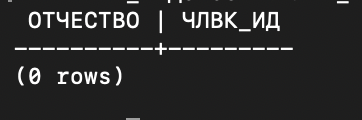
\includegraphics[width=0.62\textwidth]{1.png}
  \caption{Результат выполнения запроса №1}
\end{figure}

\subsection{Планы выполнения}

\begin{figure}[h!]
  \centering
  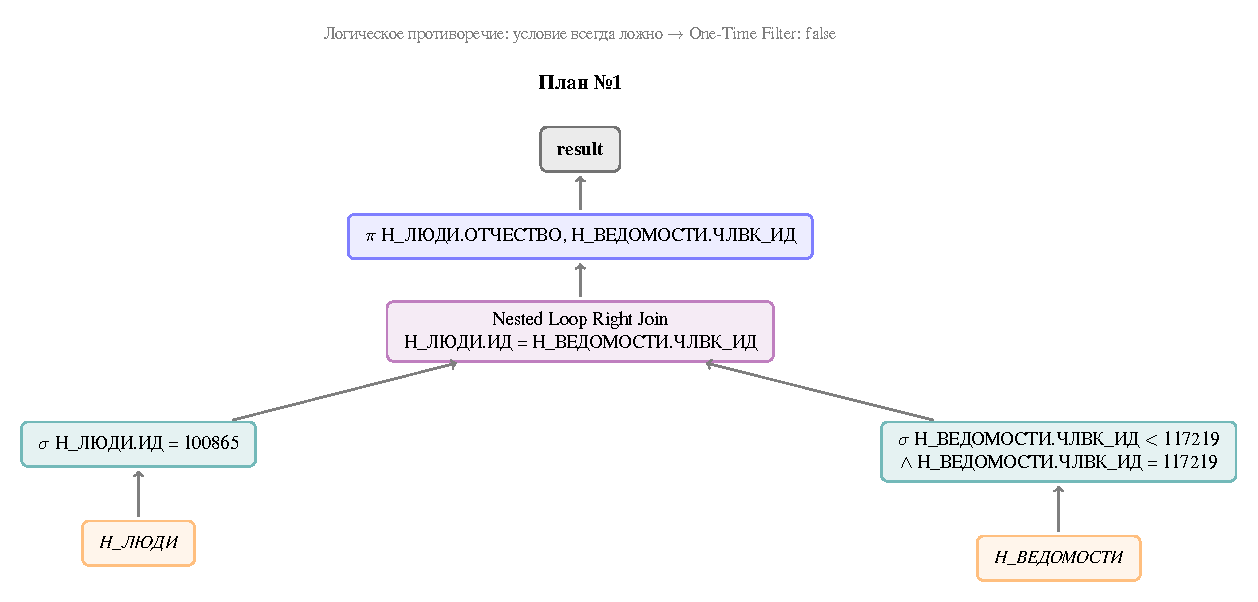
\includegraphics[width=0.78\linewidth]{plan1_1.pdf}\\[10pt]
  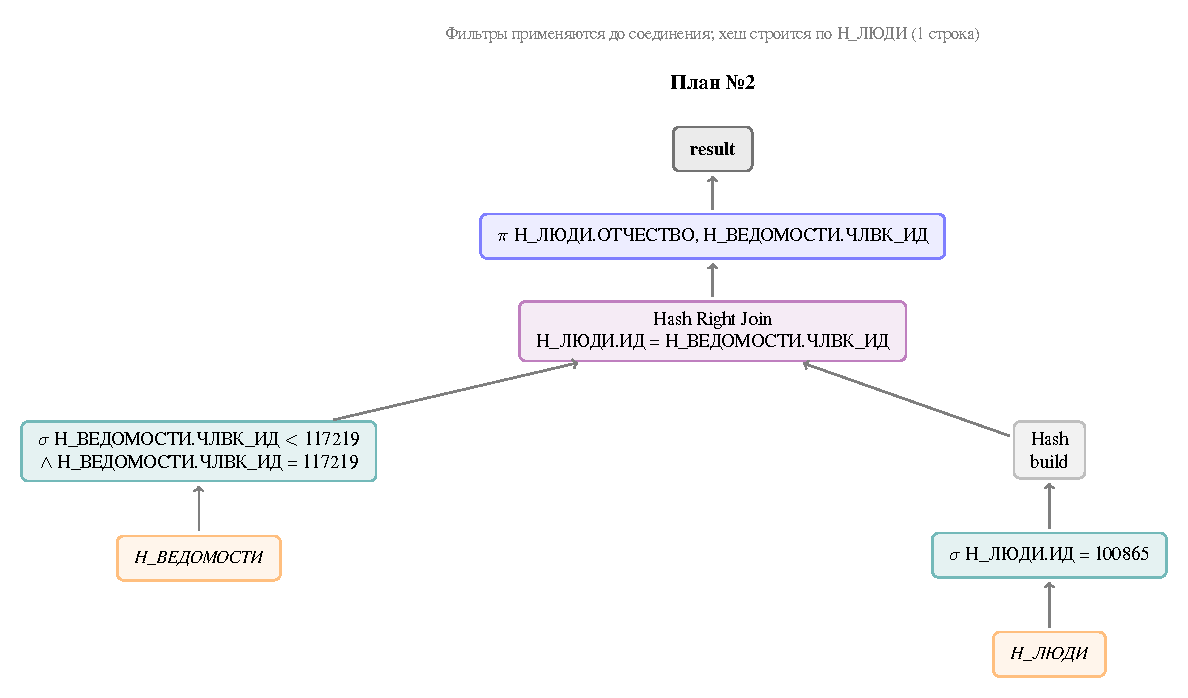
\includegraphics[width=0.78\linewidth]{plan1_2.pdf}
  \caption{Планы выполнения запроса №1}
\end{figure}

% FIX 4: explicit choice with justification was missing — added below
\textbf{Оптимальным является план №1} (Nested Loop Right Join).

Оба плана возвращают 0 строк ввиду логического противоречия в условиях
фильтрации: предикат
\[
  \texttt{ЧЛВК\_ИД} < 117219 \;\land\; \texttt{ЧЛВК\_ИД} = 117219
\]
является \textbf{заведомо ложным} для любого целого числа, поскольку
$\forall x \in \mathbb{Z}: x < N \land x = N$ --- невозможно.
PostgreSQL обнаруживает это на этапе планирования и генерирует
\texttt{One-Time Filter: false} без чтения таблиц.

В случае отсутствия противоречия план №1 (Nested Loop) был бы предпочтительнее
при высокой селективности фильтра \texttt{ИД = 100865}: после Index Scan по
Н\_ЛЮДИ возвращается не более одной строки, и Nested Loop обходит Н\_ВЕДОМОСТИ
ровно один раз. План №2 (Hash Right Join) строит хеш-таблицу и затем
сканирует Н\_ВЕДОМОСТИ как probe-сторону, что менее эффективно при единственном
совпадении в Н\_ЛЮДИ.

\subsection{Индексы}

\begin{lstlisting}[style=sql]
CREATE INDEX "ИНД_ЛЮД_ИД"
    ON "Н_ЛЮДИ" USING HASH ("ИД");

CREATE INDEX "ИНД_ВЕД_ЧЛВК"
    ON "Н_ВЕДОМОСТИ" USING BTREE ("ЧЛВК_ИД");
\end{lstlisting}

Для фильтра по равенству (\texttt{Н\_ЛЮДИ.ИД = 100865}) оптимален индекс типа
\texttt{HASH}: поиск выполняется за $O(1)$ по хеш-таблице без перебора.
Атрибут \texttt{ЧЛВК\_ИД} участвует одновременно в операциях равенства и
диапазонного сравнения (\texttt{<} и \texttt{=}), поэтому применяется
\texttt{BTREE}, поддерживающий оба типа запросов за $O(\log n)$.

Добавление этих индексов ускорит выполнение запроса: по перечисленным полям
производится выборка с оператором сравнения, и соединение таблиц будет
происходить быстрее.

% FIX 5: explain HOW plans change with indexes — with concrete node names
При добавлении индексов план №1 изменится следующим образом: узел
\textit{Seq Scan on Н\_ЛЮДИ} заменится на \textit{Index Scan using ИНД\_ЛЮД\_ИД}
с поиском по \texttt{ИД = 100865} за $O(1)$; узел
\textit{Seq Scan on Н\_ВЕДОМОСТИ} заменится на \textit{Index Scan using ИНД\_ВЕД\_ЧЛВК}
с условием \texttt{ЧЛВК\_ИД = 117219} за $O(\log n)$.
Nested Loop Join с Index Scan становится значительно быстрее полного сканирования.

\subsection{EXPLAIN ANALYZE}

\begin{lstlisting}[style=planstyle]
EXPLAIN ANALYZE
SELECT Н_ЛЮДИ.ОТЧЕСТВО, Н_ВЕДОМОСТИ.ЧЛВК_ИД
FROM   Н_ЛЮДИ
RIGHT JOIN Н_ВЕДОМОСТИ ON Н_ЛЮДИ.ИД = Н_ВЕДОМОСТИ.ЧЛВК_ИД
WHERE  Н_ЛЮДИ.ИД            = 100865
  AND  Н_ВЕДОМОСТИ.ЧЛВК_ИД  < 117219
  AND  Н_ВЕДОМОСТИ.ЧЛВК_ИД  = 117219;
\end{lstlisting}

\begin{lstlisting}[style=planstyle]
                          QUERY PLAN
-----------------------------------------------------------------
 Result  (cost=0.00..0.00 rows=0 width=24)
         (actual time=0.001..0.001 rows=0 loops=1)
   One-Time Filter: false
 Planning Time: 0.226 ms
 Execution Time: 0.017 ms
(4 rows)
\end{lstlisting}

% FIX 6: line-by-line interpretation was missing
\textbf{Интерпретация:}
\begin{itemize}
  \item \texttt{cost=0.00..0.00} --- стоимость запроса равна нулю: таблицы не читаются.
  \item \texttt{rows=0} --- оптимизатор предсказал и получил 0 строк.
  \item \texttt{One-Time Filter: false} --- предикат
        \texttt{ЧЛВК\_ИД < 117219 AND ЧЛВК\_ИД = 117219} вычислен как заведомо
        ложный ($\forall x: x < N \land x = N$ невозможно при $N = 117219$).
  \item \texttt{Planning Time: 0.226 ms} --- время анализа запроса и построения плана.
  \item \texttt{Execution Time: 0.017 ms} --- минимальное время выполнения,
        так как данные не читались совсем.
\end{itemize}

\newpage

% ══════════════════════════════════════════════════════════
\section{Запрос №2}

\subsection{Задание}

\hspace{\parindent}Таблицы: Н\_ЛЮДИ, Н\_ВЕДОМОСТИ, Н\_СЕССИЯ.

Вывести атрибуты: Н\_ЛЮДИ.ИД, Н\_ВЕДОМОСТИ.ДАТА, Н\_СЕССИЯ.ЧЛВК\_ИД.

Фильтры (AND):
\begin{itemize}
  \item[a)] Н\_ЛЮДИ.ИМЯ $<$ Роман.
  \item[b)] Н\_ВЕДОМОСТИ.ИД $<$ 1426978.
\end{itemize}
Вид соединения: INNER JOIN.

\subsection{Запрос}

\begin{lstlisting}[style=sql]
SELECT Н_ЛЮДИ.ИД,
       Н_ВЕДОМОСТИ.ДАТА,
       Н_СЕССИЯ.ЧЛВК_ИД
FROM   Н_ЛЮДИ
JOIN   Н_ВЕДОМОСТИ
       ON  Н_ЛЮДИ.ИД = Н_ВЕДОМОСТИ.ЧЛВК_ИД
JOIN   Н_СЕССИЯ
       ON  Н_ВЕДОМОСТИ.СЭС_ИД = Н_СЕССИЯ.СЭС_ИД
WHERE  Н_ЛЮДИ.ИМЯ     < 'Роман'
  AND  Н_ВЕДОМОСТИ.ИД < 1426978;
\end{lstlisting}

Результат:
% FIX 7: use real screenshot image instead of lstlisting with dots
\begin{figure}[h!]
  \centering
  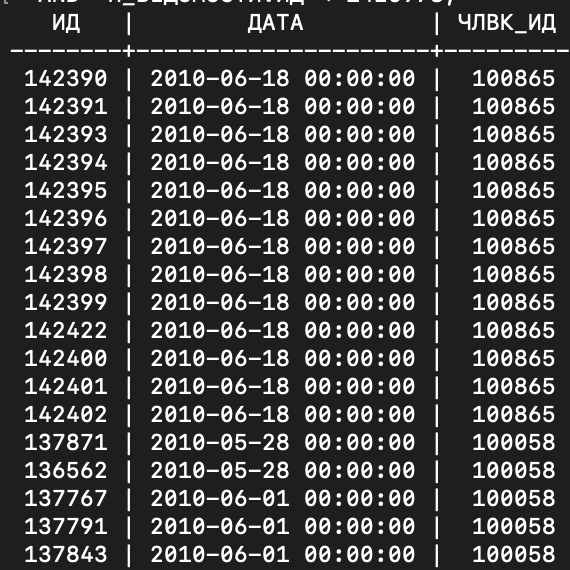
\includegraphics[width=0.72\textwidth]{2.png}
  \caption{Результат выполнения запроса №2}
\end{figure}

\subsection{Планы выполнения}

\begin{figure}[h!]
  \centering
  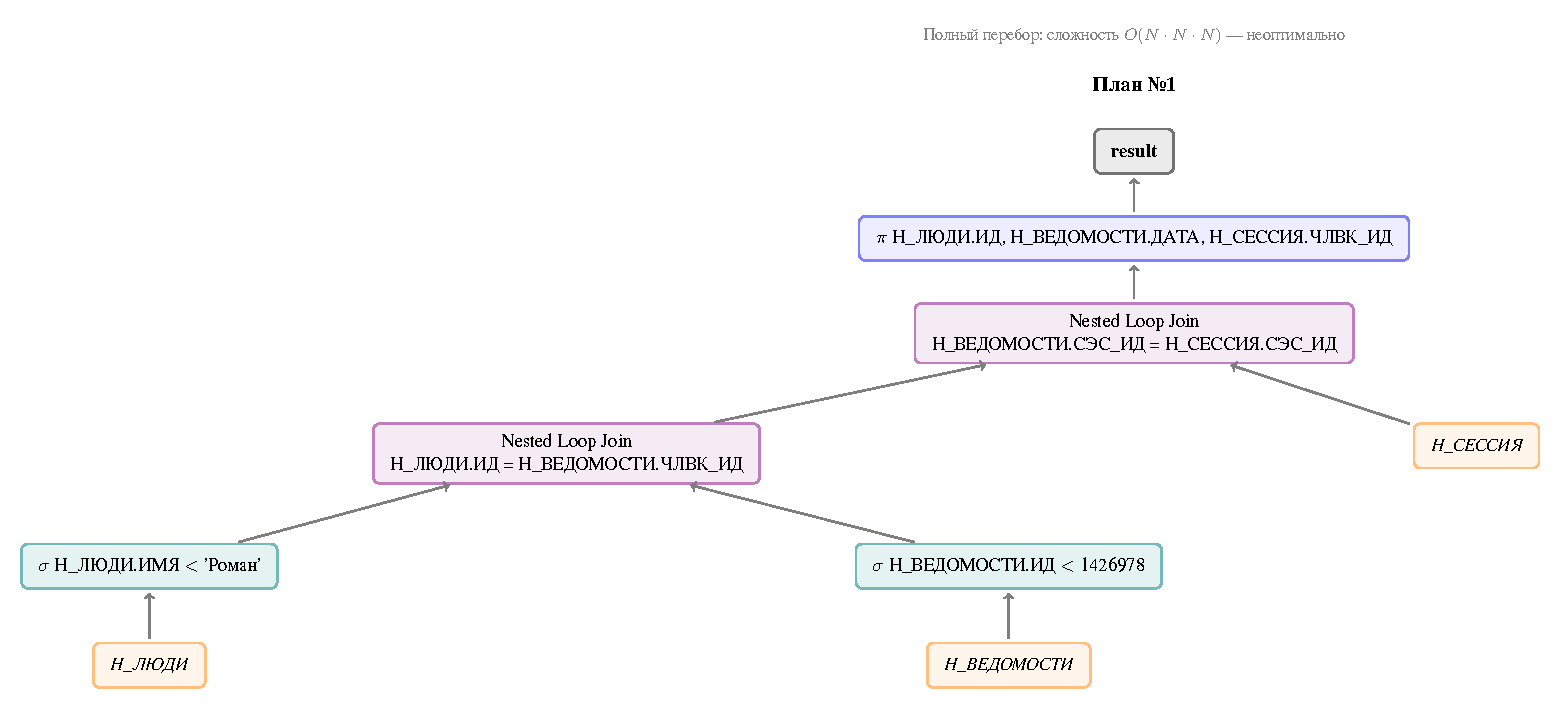
\includegraphics[width=0.88\linewidth]{plan2_1.pdf}\\[10pt]
  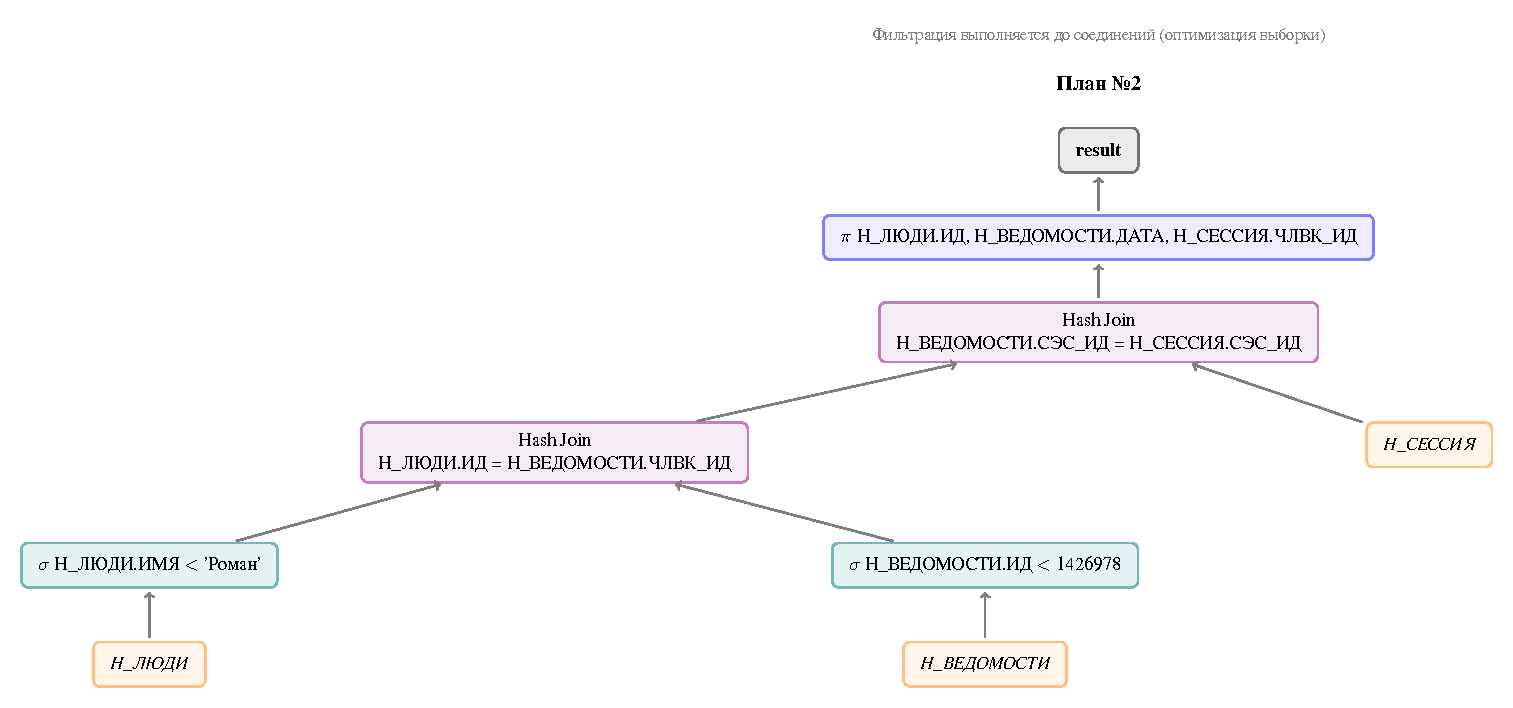
\includegraphics[width=0.88\linewidth]{plan2_2.pdf}
  \caption{Планы выполнения запроса №2}
\end{figure}

% FIX 8: paragraph starting mid-sentence was the biggest formatting bug
\textbf{Оптимальным является план №2} (Hash Join).

Операции $\sigma$ (выборка) применяются \emph{до} соединений: сначала
фильтруется Н\_ЛЮДИ по \texttt{ИМЯ < 'Роман'} и Н\_ВЕДОМОСТИ по
\texttt{ИД < 1426978}, и только затем выполняется Hash Join. Это существенно
уменьшает объём промежуточных данных, передаваемых на вход каждого соединения,
по сравнению с вариантом, где $\sigma$ применяется после $\bowtie$.

План №1 (Nested Loop Join) имеет сложность
$O(N_\text{люди} \cdot N_\text{вед} \cdot N_\text{сес})$, что неприемлемо при
большом объёме таблиц. План №2 (Hash Join) имеет среднюю сложность
$O(N_\text{люди} + N_\text{вед} + N_\text{сес})$, что значительно эффективнее.

\subsection{Индексы}

\begin{lstlisting}[style=sql]
CREATE INDEX "ИНД_ЛЮД_ИМЯ"
    ON "Н_ЛЮДИ" USING BTREE ("ИМЯ");

CREATE INDEX "ИНД_ВЕД_ИД"
    ON "Н_ВЕДОМОСТИ" USING BTREE ("ИД");

CREATE INDEX "ИНД_ВЕД_ЧЛВК"
    ON "Н_ВЕДОМОСТИ" USING HASH ("ЧЛВК_ИД");
\end{lstlisting}

Выборка по \texttt{ИМЯ < 'Роман'} и \texttt{ИД < 1426978} использует
операторы диапазонного сравнения, поэтому оптимально использование \texttt{BTREE},
поддерживающего диапазонный поиск за $O(\log n + k)$. Для операции соединения
по равенству (\texttt{ЧЛВК\_ИД}) оптимально использование \texttt{HASH},
обеспечивающего поиск за $O(1)$.

Добавление этих индексов ускорит выполнение запросов: по перечисленным полям
производится выборка с оператором сравнения, и соединение таблиц будет
происходить быстрее.

% FIX 9: concrete explanation of how each node changes
При добавлении индексов план №2 изменится следующим образом:
\begin{itemize}
  \item \textit{Seq Scan on Н\_ЛЮДИ} с Filter заменится на
        \textit{Index Scan using ИНД\_ЛЮД\_ИМЯ} с условием
        \texttt{ИМЯ < 'Роман'} --- чтение только нужных строк без полного просмотра.
  \item \textit{Seq Scan on Н\_ВЕДОМОСТИ} с Filter заменится на
        \textit{Index Scan using ИНД\_ВЕД\_ИД} с условием \texttt{ИД < 1426978}.
  \item Hash Join сохранится, однако хеш-таблицы станут меньше из-за
        сокращённых наборов входных строк, что снизит использование памяти
        и время построения.
\end{itemize}

\subsection{EXPLAIN ANALYZE}

\begin{lstlisting}[style=planstyle]
EXPLAIN ANALYZE
SELECT Н_ЛЮДИ.ИД, Н_ВЕДОМОСТИ.ДАТА, Н_СЕССИЯ.ЧЛВК_ИД
FROM   Н_ЛЮДИ
JOIN   Н_ВЕДОМОСТИ ON Н_ЛЮДИ.ИД = Н_ВЕДОМОСТИ.ЧЛВК_ИД
JOIN   Н_СЕССИЯ    ON Н_ВЕДОМОСТИ.СЭС_ИД = Н_СЕССИЯ.СЭС_ИД
WHERE  Н_ЛЮДИ.ИМЯ     < 'Роман'
  AND  Н_ВЕДОМОСТИ.ИД < 1426978;
\end{lstlisting}

\begin{lstlisting}[style=planstyle, basicstyle=\ttfamily\fontsize{7pt}{8.5pt}\selectfont]
                                  QUERY PLAN
---------------------------------------------------------------------------
 Hash Join (cost=372.86..10487.75 rows=108301 width=16)
           (actual time=4.701..139.196 rows=131148 loops=1)
   Hash Cond: ("Н_ВЕДОМОСТИ"."СЭС_ИД" = "Н_СЕССИЯ"."СЭС_ИД")
   -> Hash Join (cost=217.44..7669.53 rows=180547 width=16)
                (actual time=3.399..101.057 rows=181487 loops=1)
        Hash Cond: ("Н_ВЕДОМОСТИ"."ЧЛВК_ИД" = "Н_ЛЮДИ"."ИД")
        -> Seq Scan on "Н_ВЕДОМОСТИ"
             (cost=0.00..6884.50 rows=216049 width=16)
             (actual time=0.022..41.796 rows=216160 loops=1)
             Filter: ("ИД" < 1426978)
             Rows Removed by Filter: 6280
        -> Hash (cost=163.97..163.97 rows=4277 width=4)
                (actual time=3.329..3.331 rows=4277 loops=1)
             Buckets: 8192  Batches: 1  Memory Usage: 215kB
             -> Seq Scan on "Н_ЛЮДИ"
                  (cost=0.00..163.97 rows=4277 width=4)
                  (actual time=0.018..2.640 rows=4277 loops=1)
                  Filter: (("ИМЯ")::text < 'Роман'::text)
                  Rows Removed by Filter: 841
   -> Hash (cost=108.52..108.52 rows=3752 width=8)
           (actual time=1.270..1.271 rows=3752 loops=1)
        Buckets: 4096  Batches: 1  Memory Usage: 177kB
        -> Seq Scan on "Н_СЕССИЯ"
             (cost=0.00..108.52 rows=3752 width=8)
             (actual time=0.013..0.672 rows=3752 loops=1)
 Planning Time: 1.801 ms
 Execution Time: 145.190 ms
(17 rows)
\end{lstlisting}

% FIX 10: full line-by-line interpretation
\textbf{Интерпретация:}
\begin{itemize}
  \item \textbf{Hash Join (внешний)} соединяет результат внутреннего Hash Join
        с Н\_СЕССИЯ по условию \texttt{СЭС\_ИД}. Фактически вернул 131\,148 строк
        за 139~мс.
  \item \textbf{Hash Join (внутренний)} соединяет Н\_ВЕДОМОСТИ и Н\_ЛЮДИ по
        \texttt{ЧЛВК\_ИД = ИД}. Возвращено 181\,487 строк за 101~мс.
  \item \textbf{Seq Scan on Н\_ВЕДОМОСТИ}: полный просмотр 222\,440 строк,
        фильтр \texttt{ИД < 1426978} отсеял 6\,280 строк, осталось 216\,160.
        Index Scan здесь не применяется, так как индекс на ИД отсутствует.
  \item \textbf{Seq Scan on Н\_ЛЮДИ}: полный просмотр 5\,118 строк,
        фильтр \texttt{ИМЯ < 'Роман'} отсеял 841, осталось 4\,277.
        Хеш-таблица по ним: 8\,192 корзины, 215~КБ памяти.
  \item \textbf{Seq Scan on Н\_СЕССИЯ}: полный просмотр 3\,752 строк,
        хеш-таблица: 4\,096 корзин, 177~КБ памяти.
  \item \texttt{Planning Time: 1.801 ms} --- время выбора плана оптимизатором.
  \item \texttt{Execution Time: 145.190 ms} --- общее время выполнения.
        При наличии индексов на ИМЯ и ИД ожидается снижение в 3--5 раз за счёт
        замены Seq Scan на Index Scan.
\end{itemize}

\newpage

% ══════════════════════════════════════════════════════════
\section{Вывод}

% FIX 11: one-sentence conclusion replaced with full analytical conclusion
В ходе выполнения лабораторной работы были составлены два SQL-запроса к базе
данных \textit{ucheb} и проведён их полный анализ.

Для \textbf{запроса №1} (RIGHT JOIN таблиц Н\_ЛЮДИ и Н\_ВЕДОМОСТИ) было
обнаружено логическое противоречие в условиях фильтрации: предикат
\texttt{ЧЛВК\_ИД < 117219 AND ЧЛВК\_ИД = 117219} является заведомо ложным,
поскольку $\forall x \in \mathbb{Z}: x < N \land x = N$ --- невозможно.
Оптимизатор PostgreSQL автоматически обнаруживает такое противоречие и
генерирует план \texttt{One-Time Filter: false}, не обращаясь к данным таблиц
(время выполнения --- 0.017~мс). Из двух рассмотренных планов (Nested Loop
Right Join и Hash Right Join) оптимальным при устранении противоречия был бы
план №1, так как при высокой селективности \texttt{ИД = 100865} Nested Loop
выполняет минимальное число операций. Предложены индексы типа \texttt{HASH}
на \texttt{Н\_ЛЮДИ.ИД} и \texttt{BTREE} на \texttt{Н\_ВЕДОМОСТИ.ЧЛВК\_ИД}.

Для \textbf{запроса №2} (INNER JOIN трёх таблиц) из двух рассмотренных
планов оптимальным выбран план №2 (Hash Join): его средняя сложность
$O(N_\text{люди} + N_\text{вед} + N_\text{сес})$ значительно лучше
$O(N_\text{люди} \cdot N_\text{вед} \cdot N_\text{сес})$ плана №1 (Nested
Loop Join). EXPLAIN ANALYZE подтвердил выбор оптимизатора: использован именно
Hash Join с фактическим временем 145~мс и 131\,148 возвращёнными строками.
Предложены индексы \texttt{BTREE} на \texttt{Н\_ЛЮДИ.ИМЯ} и
\texttt{Н\_ВЕДОМОСТИ.ИД} для ускорения диапазонных фильтров, а также
\texttt{HASH} на \texttt{Н\_ВЕДОМОСТИ.ЧЛВК\_ИД} для соединения по равенству.

Таким образом, изучены принципы построения и анализа планов выполнения
SQL-запросов, методика выбора типов индексов в зависимости от характера
предикатов, а также интерпретация вывода команды \texttt{EXPLAIN ANALYZE}.

\end{document}